\documentclass[tikz,border=8pt]{standalone}
% Shared look for every TikZ diagram. Load with \input{../../tools/tikz-style.tex}
\usepackage[T1]{fontenc}
\usepackage{lmodern}
\renewcommand{\sfdefault}{lmr}  % diagrams use the same serif as the text
\usetikzlibrary{arrows.meta, positioning, shapes.geometric, calc, fit, backgrounds}
\definecolor{cblue}{HTML}{4C78A8}
\definecolor{corange}{HTML}{F58518}
\definecolor{cgreen}{HTML}{54A24B}
\definecolor{cred}{HTML}{E45756}
\definecolor{cpurple}{HTML}{B279A2}
\definecolor{cgrey}{HTML}{6B6B6B}
\tikzset{
  every picture/.style={font=\sffamily, line width=1.2pt},
  box/.style={draw=#1, fill=#1!12, rounded corners=4pt, align=center, inner sep=7pt, minimum height=1.1cm},
  box/.default=cgrey,
  arrow/.style={-{Stealth[length=3mm]}, draw=cgrey, line width=1.4pt},
  title/.style={font=\sffamily\bfseries\Large},
  note/.style={font=\sffamily\small, text=cgrey, align=center},
}
\AtBeginDocument{\hyphenpenalty=10000 \exhyphenpenalty=10000}

\begin{document}
\begin{tikzpicture}[every node/.style={font=\normalsize}]
  \node (g) {$\underbrace{\dfrac{\partial L}{\partial \beta}}_{m \times 1}$};
  \node[right=0.2cm of g] (eq) {$=\ -\dfrac{2}{n}$};
  \node[right=0.1cm of eq] (xt) {$\underbrace{X^{\mathsf T}}_{m \times n}$};
  \node[right=0.1cm of xt] (e) {$\underbrace{(y - \hat{y})}_{n \times 1}$};
  \node[right=1cm of e, align=left, font=\small, text=cgrey] {one row per coefficient:\\for coefficient $j$, the errors are\\multiplied by column $j$ of $X$, summed,\\and divided by $n$};
\end{tikzpicture}
\end{document}
